\documentclass[slovene,11pt,a4paper]{article}
%\usepackage{fullpage}

%dodatni paketki:
\usepackage{graphicx}
\usepackage{amsmath,amsfonts,amsthm} %matematicni paket
\usepackage{color} % omogoča barvno pisanje
\usepackage[utf8]
{inputenc}
\usepackage[slovene]{babel} % slovenski jezik/hyphenation
\usepackage{hyperref} %naredi vse povezave rečerenc, kazala,...
\numberwithin{equation}{section} % Number equations within sections (i.e. 1.1, 1.2, 2.1, 2.2 instead of 1, 2, 3, 4)
\numberwithin{figure}{section} % Number figures within sections (i.e. 1.1, 1.2, 2.1, 2.2 instead of 1, 2, 3, 4)
\numberwithin{table}{section} % Number tables within sections (i.e. 1.1, 1.2, 2.1, 2.2 instead of 1, 2, 3, 4)
\usepackage{eurosym} %za znak €




\usepackage[margin=2cm]{geometry}
\include{template}




\begin{document}
\begin{titlepage}

\newcommand{\HRule}{\rule{\linewidth}{0.5mm}} % Defines a new command for the horizontal lines, change thickness here

\center % Center everything on the page

%----------------------------------------------------------------------------------------
%	LOGO
%----------------------------------------------------------------------------------------

%\includegraphics{Logo}\\[1cm] % Include a department/university logo - this will require the graphicx package
 
%----------------------------------------------------------------------------------------


\includegraphics[width=2cm]{slike/aaa}\\[0.5cm]
 
%----------------------------------------------------------------------------------------
%	NASLOV DELA
%----------------------------------------------------------------------------------------
\textit{Univerza v Ljubljani}\\
\textit{Fakulteta za {\color{red}matematiko in fiziko}}\\[0.5cm]

\emph{Oddelek za fiziko}\\[0.5cm] % Oddelek za fiziko


%----------------------------------------------------------------------------------------
%	TITLE SECTION
%--------------------------------------------------------------------------------------
\HRule \\[0.4cm]
\huge {\bfseries 3. naloga: Numerična minimizacija}\\[0.4cm] % NASLOV SEMINARJA
\HRule \\[0.5cm] 

 \textsc{\large Poročilo pri predmetu modelska analiza 1}\\
 \textsc{\large 2015/2016}\\[1cm] % SEMINASKO DELO
 
%----------------------------------------------------------------------------------------
%	AUTHOR SECTION
%----------------------------------------------------------------------------------------



% If you don't want a supervisor, uncomment the two lines below and remove the section above
\Large \emph{Avtor:}\\
Klemen \textsc{Rahne}\\
28152028\\[2cm]
%----------------------------------------------------------------------------------------
%	DATUM
%----------------------------------------------------------------------------------------

{\large \today } \\[0.5cm] % Date, change the \today to a set date if you want to be precise

	

\end{titlepage}




%----------------------------------------------------------------------------------------
%	KAZALO
%----------------------------------------------------------------------------------------

\tableofcontents

%----------------------------------------------------------------------------------------
%	ZAČETEK TEKSTA
%----------------------------------------------------------------------------------------

\section{Thomsonov problem}
Zanima nas, kako se po površini porazdeli $N$ enakih nabojev na prevodni krogli. Naboji se poradelijo, tako, da je v dani porazdelitvi najmanjša možna elektrostatska energija:

\begin{equation}
W_{E}=\frac{1}{2}\sum_{i,j;i\neq j}^N \frac{e_0^2}{4 \pi \epsilon_0 |r_i-r_j|}
\end{equation}
Zaradi lažjega računanja bomo predpostavili $r=1$, ter vse konstante postavili na ena. Ker smo definirali $r=1$, nam v sferičnih koordinatah za opis položaja posameznega naboja ter za njegov prispevek k elektrostatski energiji ostaneta kota $\theta$ in $\phi$:
\begin{equation}
W_{E}=\frac{1}{2}\sum_{i,j;i\neq j}^N \frac{1}{\sqrt{2-2(sin\theta_i \sin\theta_j \cos(\phi_i - \phi_j)+\cos \theta_i \cos \theta_j)}}
\end{equation}
Torej bodo naše spremenljivke $N$ nabojev in $2$ kota $\phi_i, \theta_j$, skupno torej $2N$ spremenljivk. 


\subsection{Rešitve}
Problem sem reševal v programu {\tt Matlab} s klicanjem funkcije fminsearch. Na naslednji strani (slika \ref{slika-naboji1}) si lahko grafično ogledamo, kako se za različno število nabojev porazdelijo naboji po sferi.\\
V mojem programi sem najprej naboje enakomerno po kotih razporedil po površini:
\begin{equation*}
\begin{aligned}
\phi_i & =\frac{2\pi}{N}i \\
\theta_i & =\frac{\pi}{N}i
\end{aligned}
\end{equation*}
Po končani optimizaciji sem vse kote pretransformiral tako, da je bil prvi naboj vedno na severnem polu sfere. V primeru, da sem vse naboje na začetku postavil v isto točko, je na koncu optimizacije prihajalo do majhnih odstopanj v primerjavi kot, če smo jim kote enakomerno porazdelili. s primerjavo minimalne energije med, tema metodama s internetnim virom, sem ugotovil, da je metoda z enakomerno porazdeljenimi koti bolj točna.



\begin{figure}[t]
\noindent\makebox[\textwidth][l]{%
\hspace{-\dimexpr\oddsidemargin+1in}%

\begin{minipage}[t]{0.5\paperwidth}
\begin{flushleft}

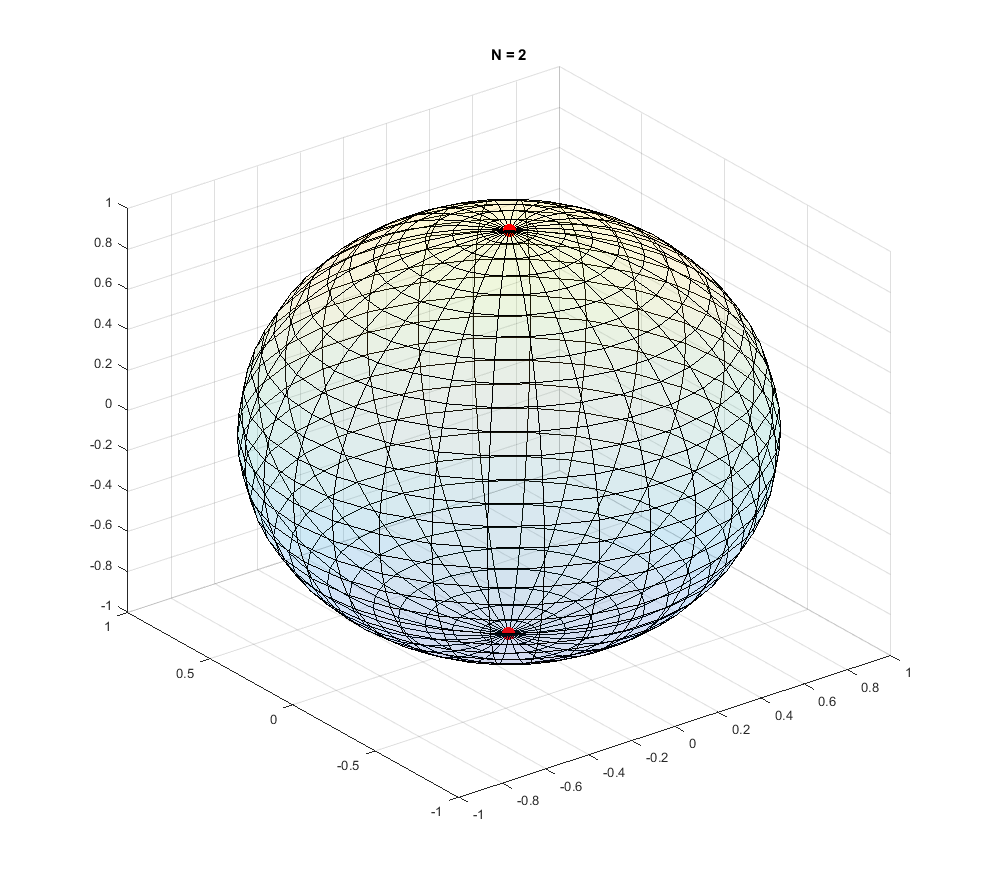
\includegraphics[scale=0.4]{slike/naboj2.png}
\hspace{\fill}
\end{flushleft}
\end{minipage}
\begin{minipage}[t]{0.5\paperwidth}
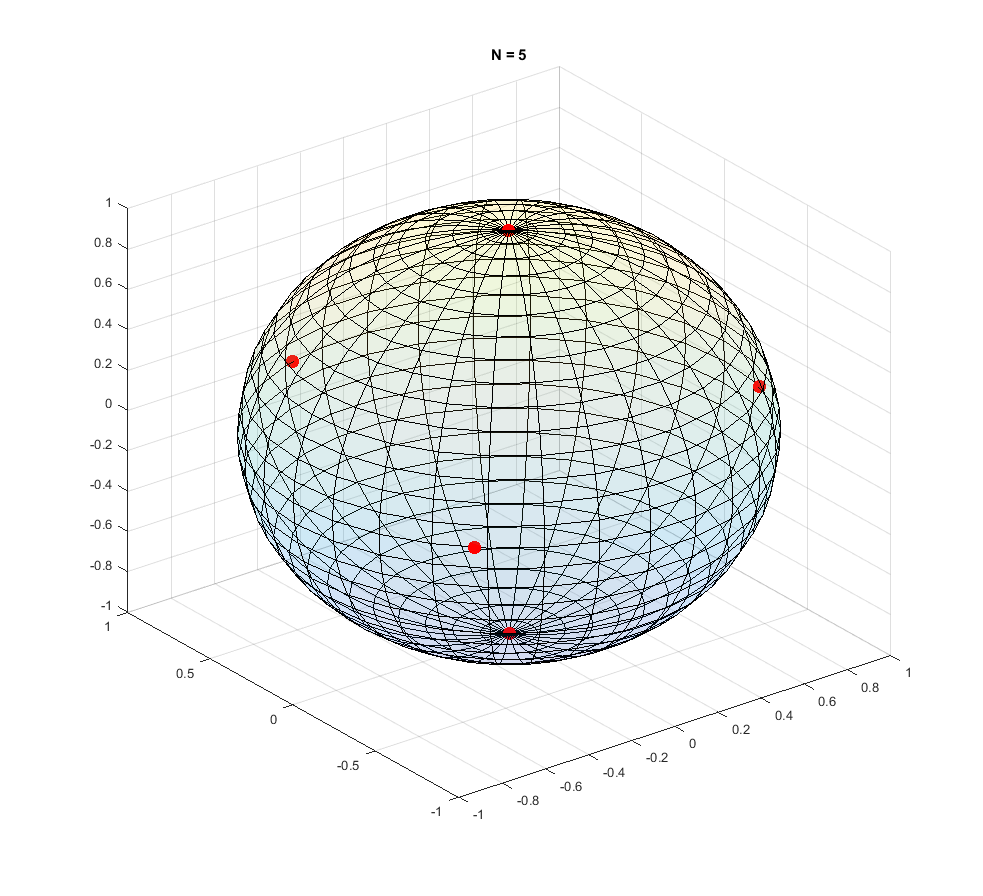
\includegraphics[scale=0.4]{slike/naboj5.png}
\end{minipage}%
}
\noindent\makebox[\textwidth][l]{%
\hspace{-\dimexpr\oddsidemargin+1in}%

\begin{minipage}[t]{0.5\paperwidth}
\begin{flushleft}

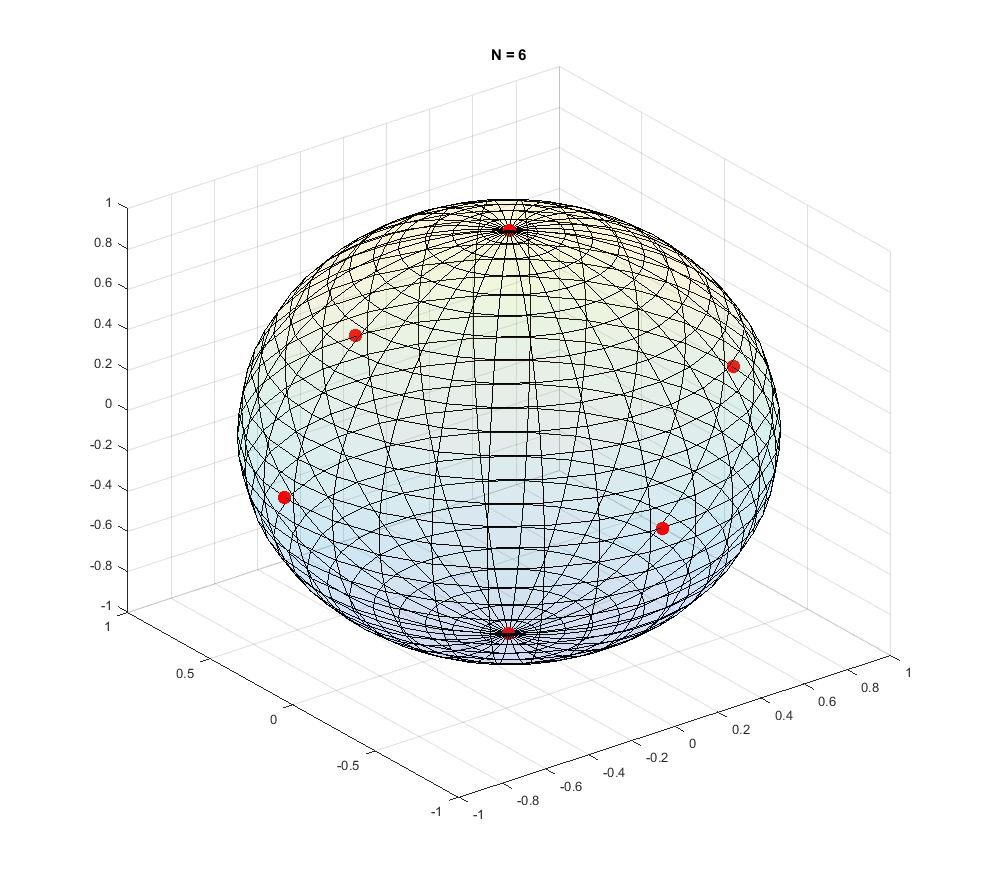
\includegraphics[scale=0.4]{slike/naboj6.png}
\hspace{\fill}
\end{flushleft}
\end{minipage}
\begin{minipage}[t]{0.5\paperwidth}
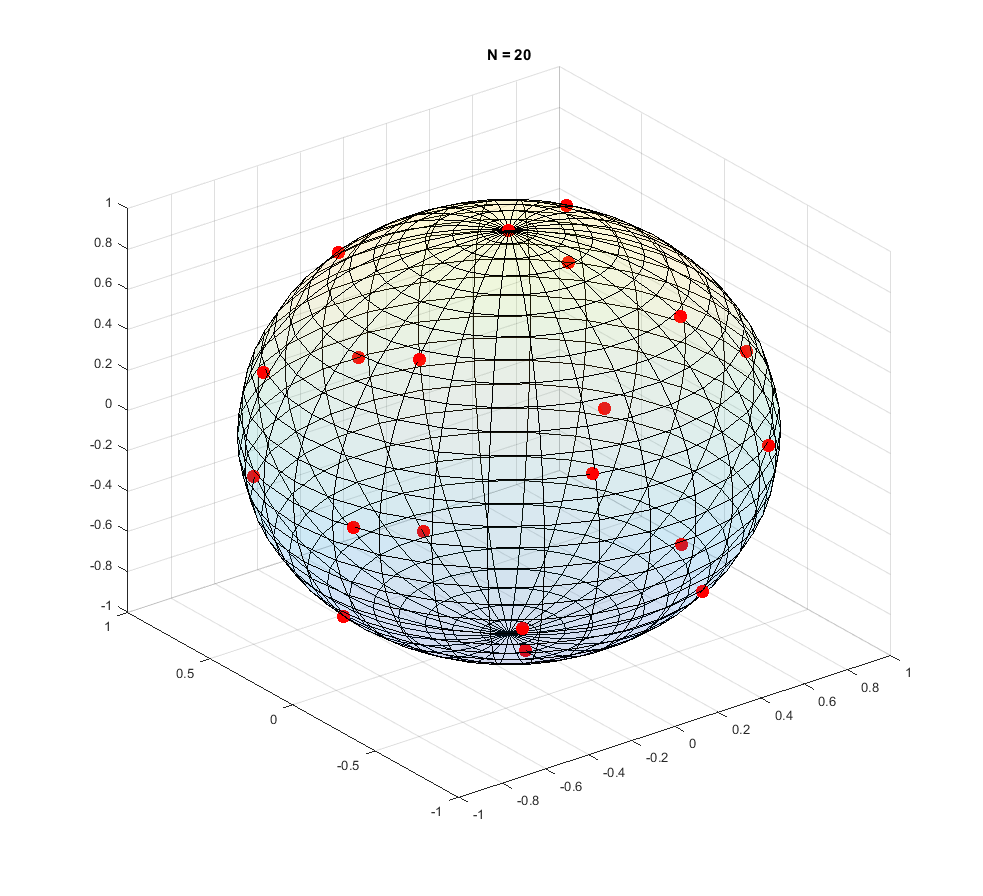
\includegraphics[scale=0.4]{slike/naboj20.png}
\end{minipage}%
}
\label{slika-naboji1}
\caption{Primeri porazdelitev nabojev za različno število nabojev. Rdeče točke ponazarjajo naboj.}
\end{figure}



\clearpage



\section{Optimalna vožnja skozi semafor}
Tako, kot v prvi nalogi, želimo optimizirati vožnjo skozi semafor :
\begin{equation}
\int_0^1 \dot{v}^2(t)dt =MIN
\end{equation}
pri pogoju: $\int_0^1 v(t) dt = 1$ (v brezdimenzijski obliki).
V prvi nalogi smo problem reševali analitično, sedaj pa bomo problem diskretizirali in reševali numerično.
Numerično integracijo opravimo po trapezni metodi:
\begin{equation}
F=\Bigg[ \frac{1}{2}(\frac{v_0 -v_{Z}}{\Delta t})^2+(\frac{v_1-v_0}{\Delta t})^2+...+\frac{1}{2} (\frac{v_N -v_{N-1}}{\Delta t})^2 \Bigg] \Delta t
\end{equation}

Uporabimo še veljavnosti vezi:
\begin{equation}
 \big( \frac{1}{2}v_0+v_1+v_2+...+v_{N-1}+\frac{1}{2}v_N \big) \Delta t=1
\end{equation}

\subsection{Prosta vožnja}
Oglejmo si primer, ko imamo podano samo začetno hitrost.

\begin{figure}[h]
\noindent\makebox[\textwidth][l]{%
\hspace{-\dimexpr\oddsidemargin+1in}%

\begin{minipage}[t]{0.5\paperwidth}
\begin{flushleft}

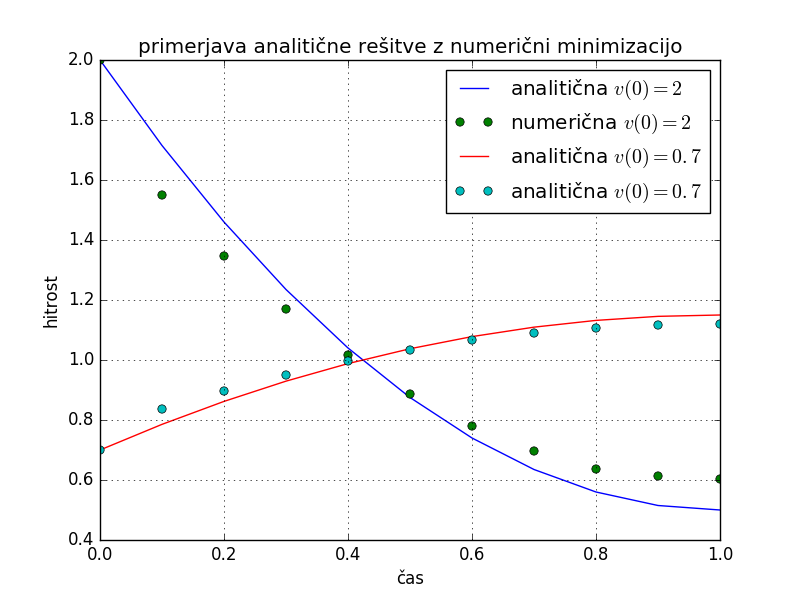
\includegraphics[scale=0.5]{slike/primerjava_anal_num_n_10.png}
%\caption{Prva stacionarna točka}
\hspace{\fill}
\end{flushleft}
\end{minipage}
\begin{minipage}[t]{0.5\paperwidth}
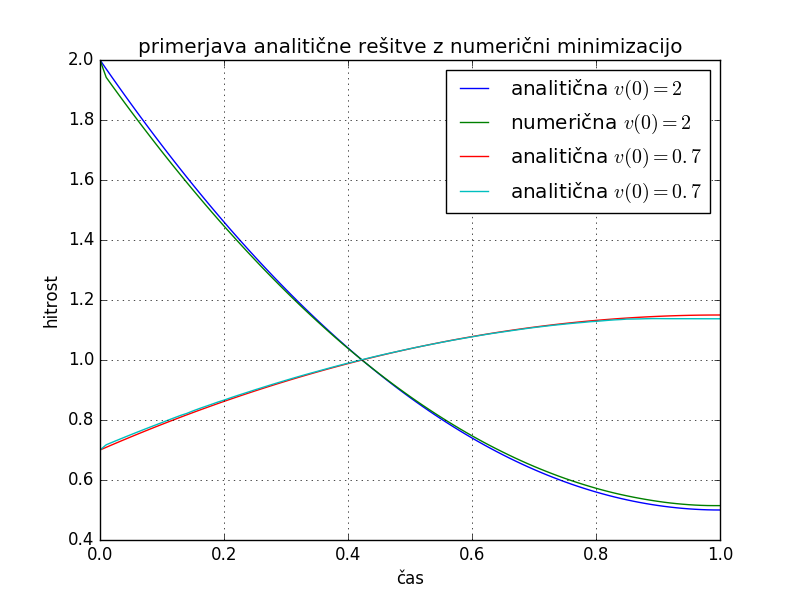
\includegraphics[scale=0.5]{slike/primerjava_anal_num_n_100.png}
%\caption{Druga stacionarna točka}
\end{minipage}%
}
\caption{Primerjava analitične rešitve z numerično. Na levem grafu vidimo, da numerična rešitev, vidno odstopa od analitične rešitve, pri $\Delta t=0.1$. Na desnem grafu, ki se od levega razlikuje le pri $\Delta t=0.01$ (desetkrat boljši časovni ločljivosti) opazimo boljše prilagajanje analitični rešitvi. Vzrok temu se najverjetneje skriva v numerični integraciji, saj z manjšanjem intervala (oz. povečanjem točk integriranja) ozboljšamo vrednost integriranja.}
\end{figure}

\pagebreak

\subsection{Fiksna končna hitrost in periodični robni pogoji}
Oglejmo si kako izgledajo rešitve, ko fiksiramo končno hitrost [$v(1)$] na neko poljubno vrednost.

\begin{figure}[h]
\noindent\makebox[\textwidth][l]{%
\hspace{-\dimexpr\oddsidemargin+1in}%

\begin{minipage}[t]{0.5\paperwidth}
\begin{flushleft}

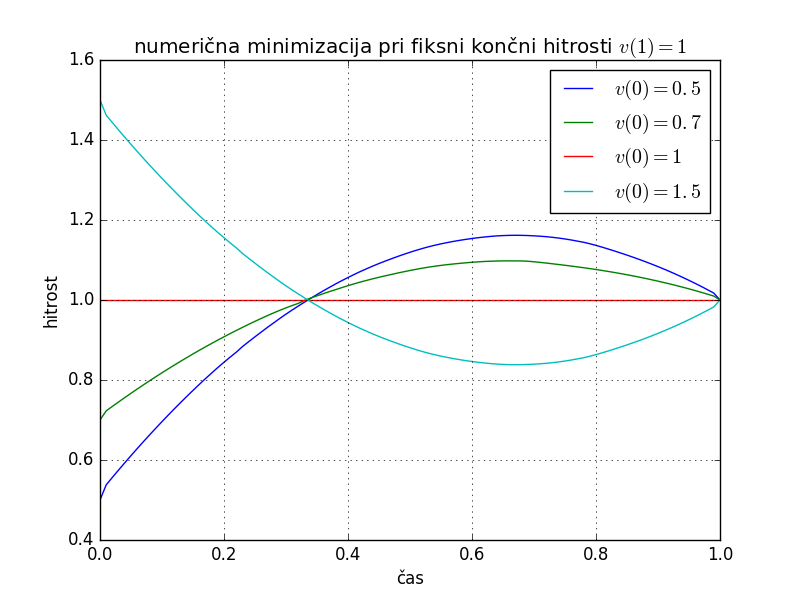
\includegraphics[scale=0.5]{slike/numericno_fiskna_koncna_n_100vk_1.png}
\hspace{\fill}
\end{flushleft}
\end{minipage}
\begin{minipage}[t]{0.5\paperwidth}
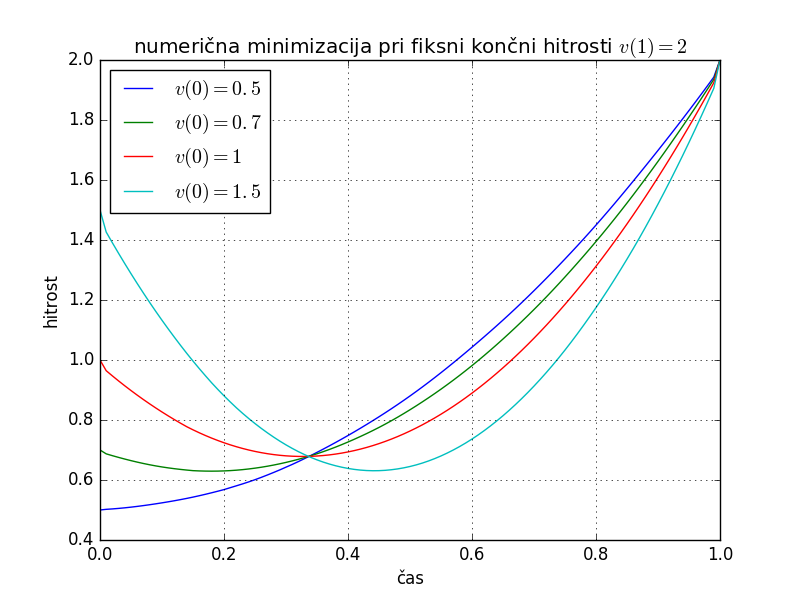
\includegraphics[scale=0.5]{slike/numericno_fiskna_koncna_n_100vk_2.png}
\end{minipage}%
}
\noindent\makebox[\textwidth][l]{%
\hspace{-\dimexpr\oddsidemargin+1in}%
\begin{minipage}[t]{0.5\paperwidth}
\begin{flushleft}

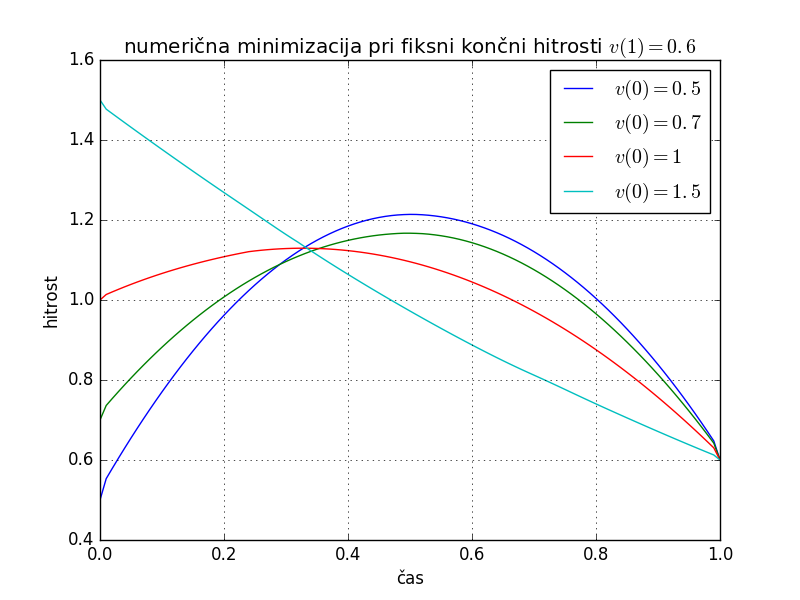
\includegraphics[scale=0.5]{slike/numericno_fiskna_koncna_n_100vk_0_6.png}
\hspace{\fill}
\end{flushleft}
\end{minipage}
\begin{minipage}[t]{0.5\paperwidth}
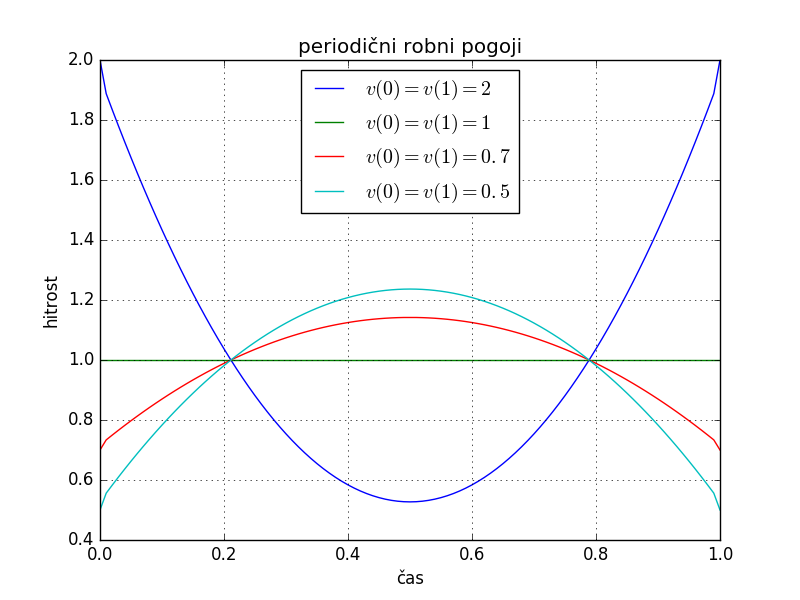
\includegraphics[scale=0.5]{slike/periodicni_robni_pogoji.png}
\end{minipage}%
}
\caption{Opazimo, da so rešitve med seboj zelo različne, odvisne od začetne in končne hitrost. Od konstantnega gibanja (graf zgoraj levo, rdeča krivulja), do približno enakomernega zaviranja (spodnji graf levo, svetlo modra krivulja), do pospeševanj in zaviranj v ostalih primerih. Poseben primer fiskne končne hitrosti je, ko je končna hitrost enaka začetni hitrost. Dobimo ti. periodični robni pogoj. To rešitev ponazarja spodnji desni graf.}
\end{figure}

\pagebreak


\subsection{Omejitev hitrost}
Za omejitev hitrosti v prvi nalogi smo poskušali z vpeljavo dodatnega člena $v(t)^2$ v integral, ki smo ga minimizirali. Ta člen smo takrat vpeljali, ker smo lahko izračunali analitično rešitev takega problema. Tokrat bomo uporabili dodatni člen oblike $e^{\beta (v-v_{max})}$.


\begin{figure}[h]
\noindent\makebox[\textwidth][l]{%
\hspace{-\dimexpr\oddsidemargin+1in}%

\begin{minipage}[t]{0.5\paperwidth}
\begin{flushleft}

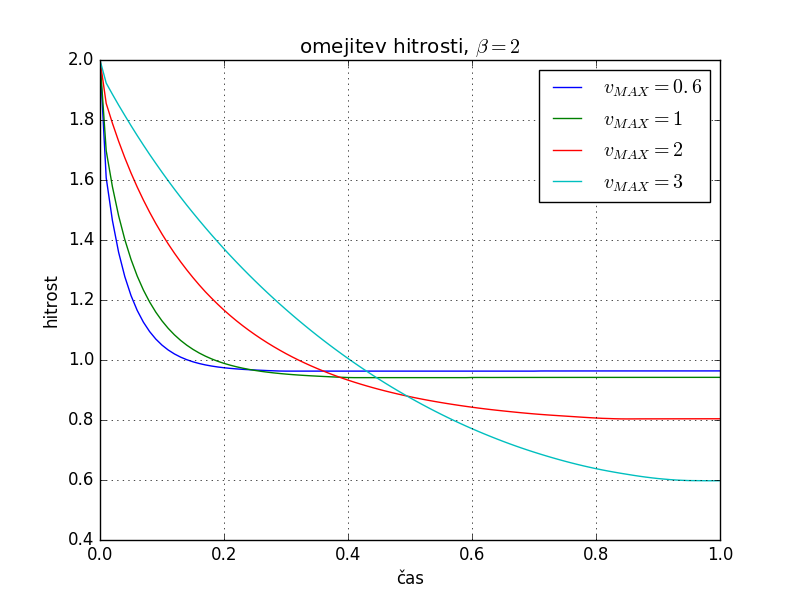
\includegraphics[scale=0.5]{slike/omejitev_hitrosti_beta_konstantna.png}
%\caption{Prva stacionarna točka}
\hspace{\fill}
\end{flushleft}
\end{minipage}
\begin{minipage}[t]{0.5\paperwidth}
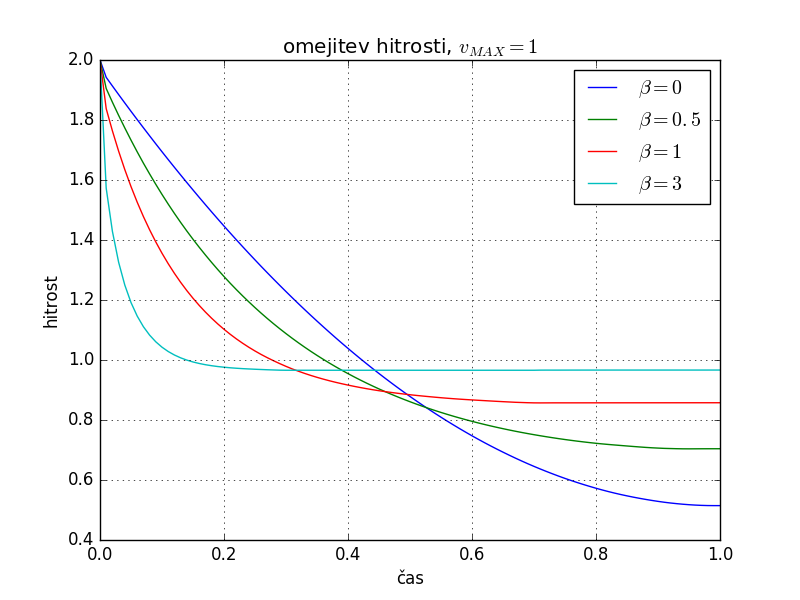
\includegraphics[scale=0.5]{slike/omejitev_hitrosti_v_max_konstantna.png}
%\caption{Druga stacionarna točka}
\end{minipage}%
}
\caption{Vpliv dodatnega člena $e^{\beta (v-v_{max})}$ k optimalni vožnji. Na levem grafu vidimo kako z večanjem največje dovoljene hitrosti ($v_{max}$) kasneje pridemo do stabilne hitrosti. V desnem grafu pa opazimo, da z naraščanjem $\beta$ hitreje pridemo k stabilni hitrosti.}
\end{figure}






%----------------------------------------------------------------------------------



\pagebreak
\end{document}
